
\section{Thesis Organization}

We are going to provide a visual map of how it all fits together: flow chart of activities, papers, and data outputs 

Fig.~\ref{intro:thesis-org:fig:essentials}

\begin{figure}[!tbp]
	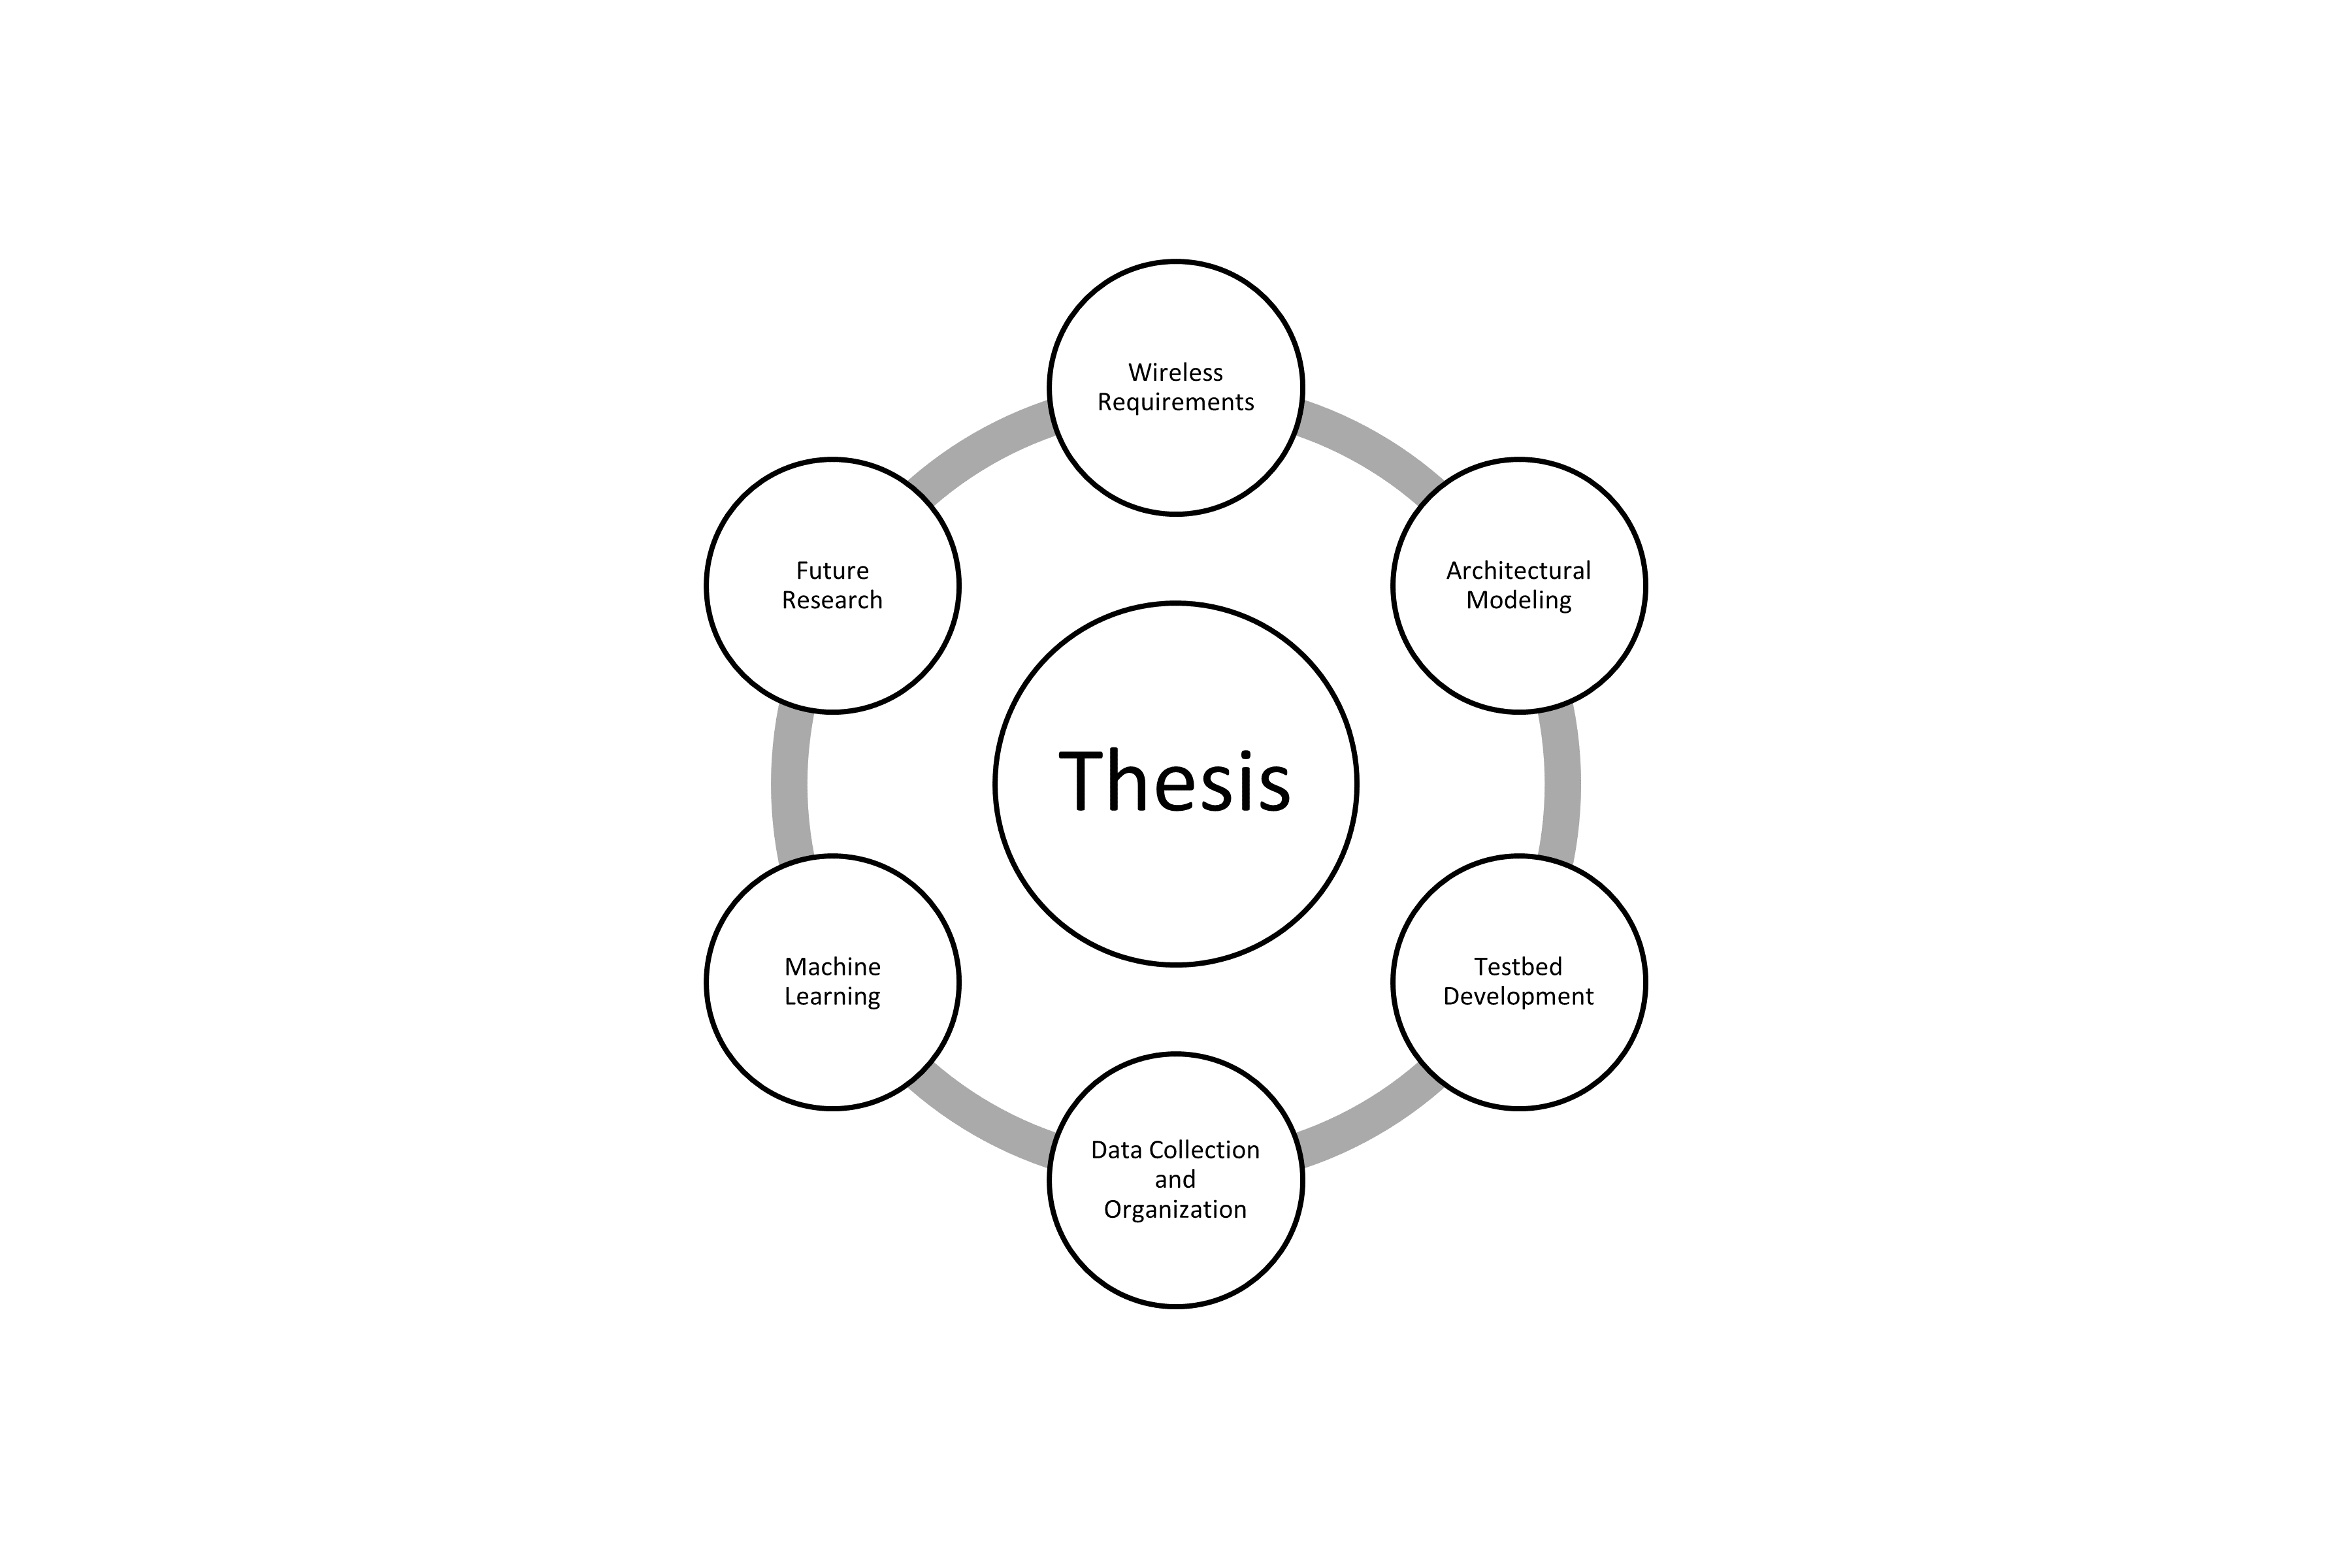
\includegraphics[width=1.0\textwidth]{chapter-intro/diagrams/Slide1}
	\caption{Essential Components of Thesis}\label{intro:thesis-org:fig:essentials}
\end{figure}


This thesis is organized to provide an inbtroduction to the world of manufacturing since the first industrial revolution to give the reader some context of where world industry has been, where it is, and where it is going.

Fig.~\ref{intro:thesis-org:fig:outline}

\begin{figure}[!tbp]
	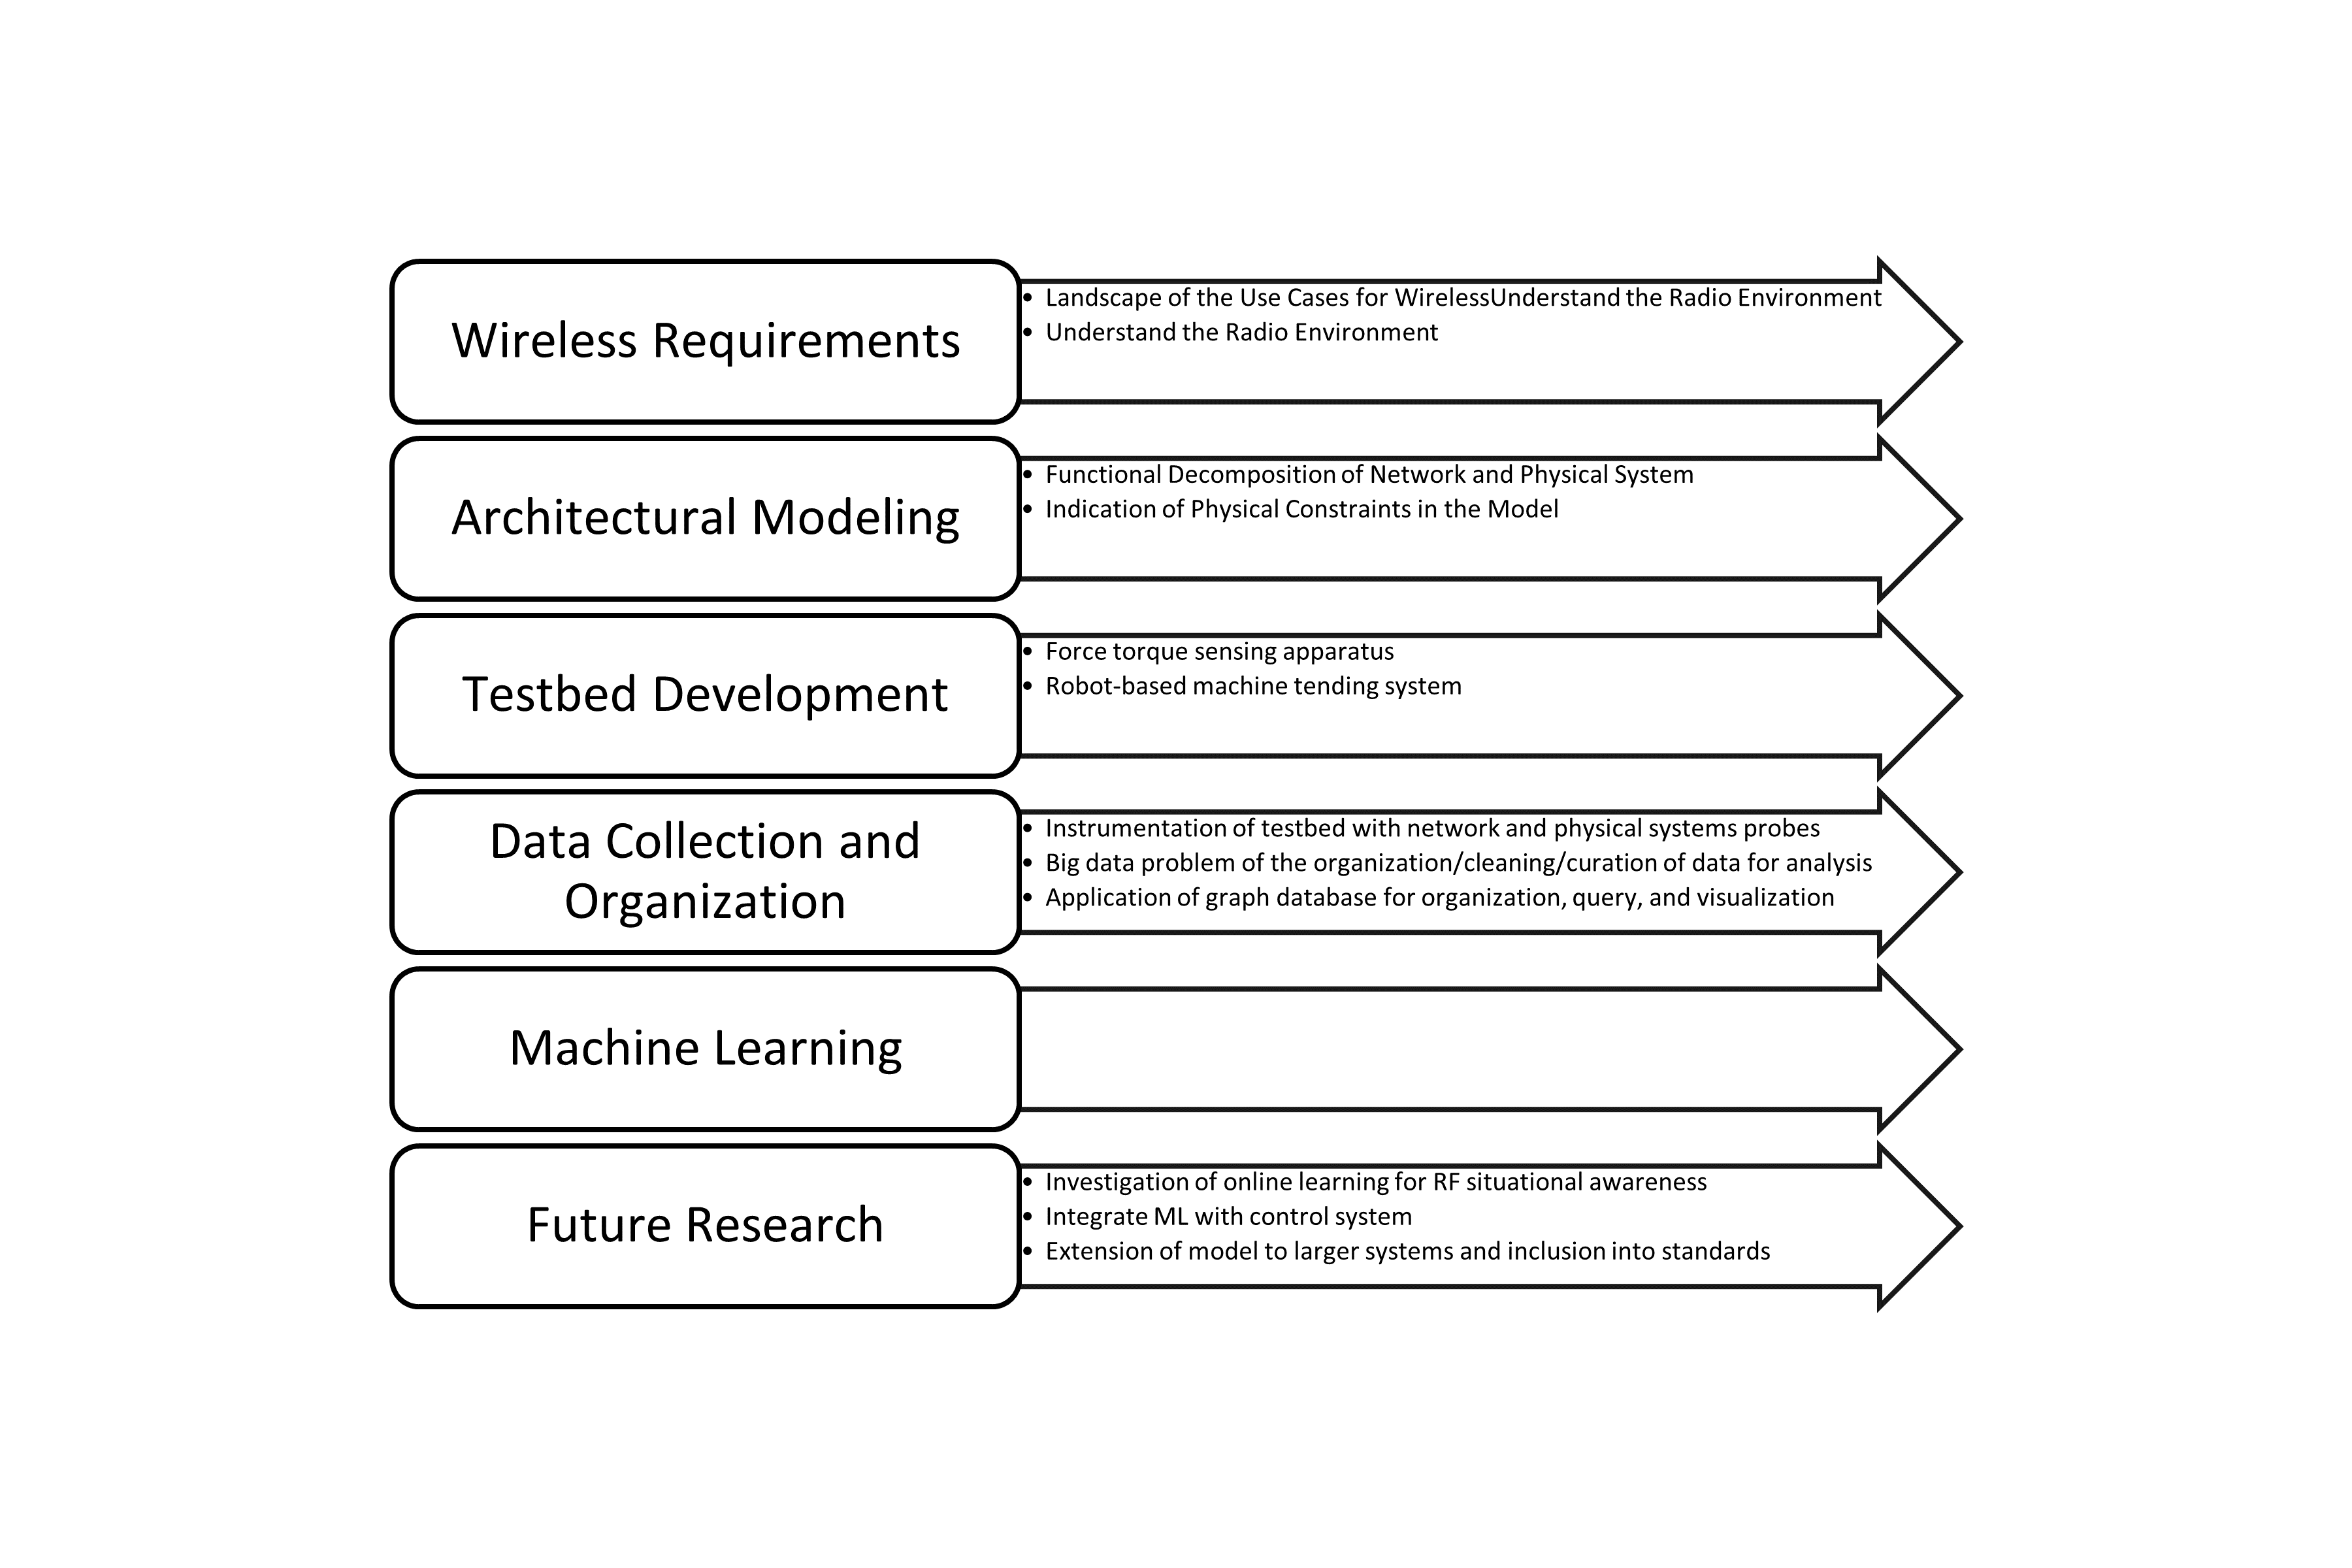
\includegraphics[width=1.0\textwidth]{chapter-intro/diagrams/Slide2}
	\caption{Essential Components of Thesis}\label{intro:thesis-org:fig:outline}
\end{figure}


Discuss the following:

SysML model in GutHub ~\cite{Candell2018SysML.GitHub}

SysML JRES Article cataloging the model~\cite{Candell2018SysML.JRES}

SysML Documentation online through Data.gov~\cite{Candell2018SysML.DATA}

